\documentclass[11pt]{amsart}

\usepackage{tgpagella}
\fontfamily{qpl}
\usepackage[utf8]{inputenc}
\usepackage{amsmath, amsthm, amscd, amsfonts, amssymb, graphicx, color}
\usepackage[bookmarksnumbered, colorlinks, plainpages=false]{hyperref}
\usepackage{bookmark}
\usepackage{csquotes}
\usepackage{dirtytalk}
\usepackage{float}

\usepackage[dutch]{babel}

\usepackage[style=verbose,backend=biber]{biblatex}
\addbibresource{zotero.bib}

\hypersetup{
     colorlinks = true,
     citecolor = blue,
     urlcolor = blue,
     linkcolor = blue,
}

\textheight 22.5truecm \textwidth 14.5truecm
\setlength{\oddsidemargin}{0.35in}\setlength{\evensidemargin}{0.35in}

\setlength{\topmargin}{-.5cm}

\begin{document}
\setcounter{page}{1}

\noindent {\small 2324-S1 werkcollege Oude Geschiedenis}\hfill     {\small \today} \\
% title, issn/data
{\small Opdracht 2: Griekse homoseksualiteit?.}\hfill
{\small } %volume, url

\centerline{}

\centerline{}

\title[Griekse Homoseksualiteit]{Griekse Homoseksualiteit in de klassieke tijd}

\author[J. Vermeltfoort]{Vermeltfoort, Jenny$^1$}

\address{$^{1}$ 3787494, Faculteit Geesteswetenschappen, Leiden
     Universiteit, Leiden, Nederland.}
\email{\textcolor[rgb]{0.00,0.00,0.84}{j.vermeltfoort@umail.leidenuniv.nl}}

%\dedicatory{This paper is dedicated to Professor ABCD}
%\subjclass[2020]{Primary 46L55; Secondary 44B20.}
%\keywords{Analysis, PDEs, algebra, number theory, applied mathematics}
%\date{Received: xxxxxx; Revised: yyyyyy; Accepted: zzzzzz.
%\newline \indent $^{*}$ Corresponding author}

\maketitle

\section*{Opdracht 1}

\noindent In de Spartaanse \textit{age classes} werden homoseksuele relaties aangemoedigd. Dit waren relaties tussen jongens
enongehuwde jongemannen en waren verbonden aan de oude initiatiepraktijken van de pubers. Deze systematische vorm van
homoseksualiteit kwam enkel in Sparta voor, maar toch werd homoseksualiteit in andere Griekse plaatsen als normaal
bevonden. Binnen de elite van Athene speelde pederastie een belangrijke
rol.\autocite{naereboutOudheidGriekenRomeinen2022}

\section*{Opdracht 2}
\noindent Op de schaal \autocite{dourisAtticRedFigure} staat een oudere man en een jongen afgebeeld. De jongen vertoont nederige
gewoontes, hij kijkt de man niet aan, en draagt zijn kledei over zijn hoofd. De oudere man houd zijn linker hand op
zijn borst en volgens de bron \autocite{dourisAtticRedFigure} heeft hij een kaalgeplukte haan in zijn hand, wat een
liefdes gift representeert. Er van uitgaande dat er werkelijk een liefdes gift word vergeven duid dit op een liefdes
relatie tussen een oudere man en een jongen, wat dus pederastie schetst.

\section*{Opdracht 3}
\noindent In figuur \ref{fig:siana-cup} \autocite{SianaCup575BC} representeert een stuk van een kop, genaamd de \textit{siana
     cup}. Er is een oudere man getoont, links, met een rode baard en een rode borst. Hij heeft zijn linkerhand op de kin
van de jongen, rechts, lang haar, geen baard, en een rode borst. De gewoontes vertonen eigenschappen van een liefdes
relatie en kan daarmee gecategoriseerd worden onder pederastie.
\begin{figure}[H]
     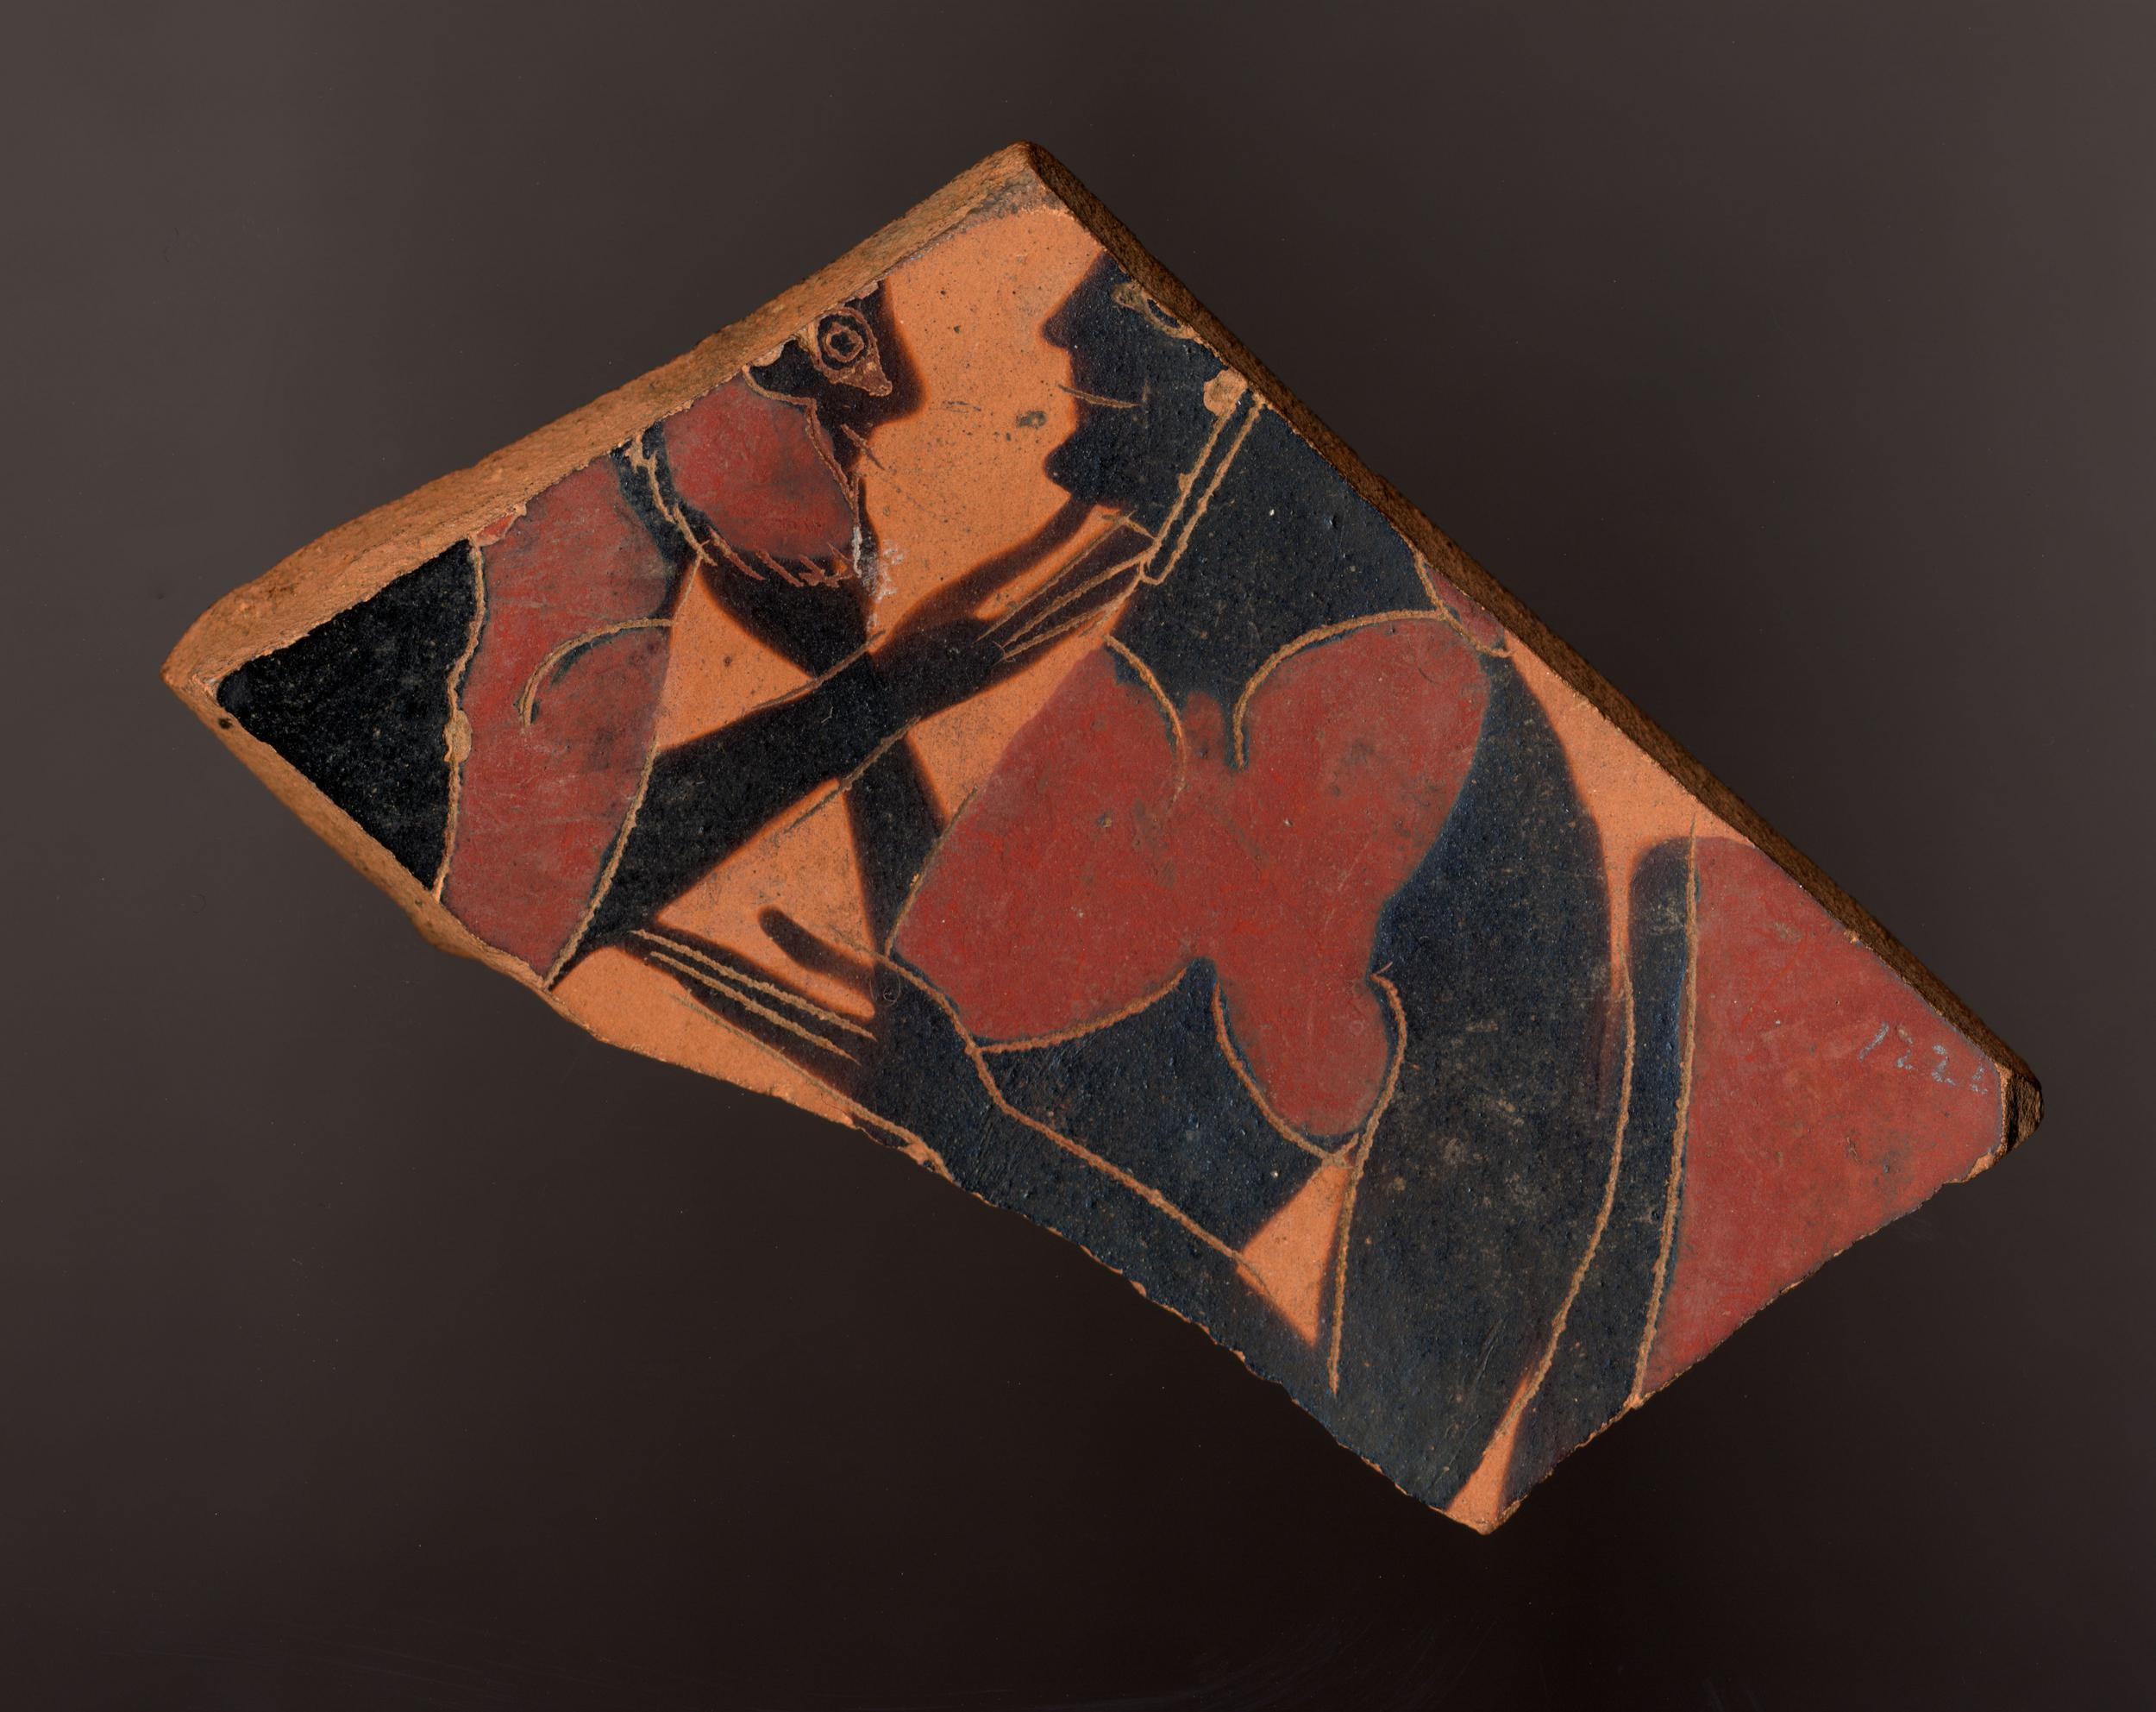
\includegraphics[width=0.5\linewidth]{images/452769001.jpg}
     \caption{Handle of Siana cup: scene of bearded man courting boy.}
     \label{fig:siana-cup}
\end{figure}

\section*{Opdracht 4}
\noindent De tekst van Plutarchus bevestigd dat in Sparta de jongemannen een oog hielden op de jongens. De jongemannen waren
\say{als het ware allemaal de vaders en opvoeders en gouverneurs van alle
     jongens.}\autocite{plutarchusLevenVanPelopidas120} Er word zelfs geconstateerd dat de liefde zorgde voor een sterke
band op het oorlogsveld, omdat \say{minnaars en beminden uit wederzijdse liefde en respect in het gevaar pal stonden
     voor elkaar.}\autocite{plutarchusLevenVanPelopidas120} Dit komt overheen met het beeld wat Naerebout en Singor over
pederastie scheppen, de gelijkenissen bluiken de \textit{age classes} maatschappij en het bevestigd dat \say{de
     homoseksualiteit hier misschien verbonden is met de resten van oude initiatiepraktijken die van de pubers mannen
     moesten maken.}\autocite{naereboutOudheidGriekenRomeinen2022}

\section*{Opdracht 5}\label{opdracht5}
\noindent Wat opvallend is aan de bron van Plutarchus \autocite{plutarchusLevenVanPelopidas120} is dat de homoseksualiteit bij de
Spartanen een bepaalde machtsspeling is. De jongens worden gekozen door oudere en status dragende jongemannen. Het is
hiermee niet geheel duidelijk of het hier om werkelijke homoseksualiteit gaat, aangezien de jongens geen andere keuze
hebben. Het hele systeem is ingebakerd in de maatschappij, het is een soort traditie of een standaard proces waar de
leden zich aan vast houden. Hierdoor komen termen zoals acceptatie in deze tijd niet voor, het is voor hun namelijk
vanzelfsprekend.

Merkbaar is dat er voornamelijk geschreven wordt over mannen met status, homoseksualiteit binnen de rest van het volk
word hier uitgesloten. Is dit echter indicatief dat de rest van de bevolking geen homoseksuele relaties ondervond, of
is dit een gevolg van het karakter van de histografie van deze tijd, waar er enkel geschreven werd over mannen met
aanzien.

\section*{Opdracht 6}
De mens was van oorsprong een gedaante met vier benen, vier armen en twee gezichten. Er waren drie seksen, man-man, vrouw-vrouw en man-vrouw, opeenvolgend representerend, de zon, de aarde en de maan.
Deze gedaantes waren bandeloos en daarom besloot Zeus ze te splitsen. Hieruit onstond de mens met twee benen. Aangezien de mens nu een helft is van haar gedaante kwam de behoefte om weer geheel te worden op.
Dit is de oorsprong van liefde, waar het gesplitse resultaat van de man-man zocht naar een mannelijke wederhelft, de vrouw-vrouw zocht naar een vrouwelijke wederhelft en de man-vrouw zocht naar een heteroseksueele wederhelft. \autocite{platoSymposium189d-193a}
Wat Aristophanes in \textit{Symposium} beredeneerd is dat de beste mannen voortkomen uit het man-man gedaante, aangezien \say{zij van nature het mannelijkst zijn}\autocite{platoSymposium189d-193a}.

\section*{Opdracht 7}
Wat geconcludeerd kan worden uit de teskt van Aristophanes is dat de homoseksuele liefde in Athene geen sociaal construct is zoals dat in Sparta is. De homoseksualiteit wordt gedefineerd als het verlangen naar een wederhelft van hetzelfde geslacht.
Zijn blik op de man-man kan verklaren hoe er gekeken werd naar de homoseksualiteit van de aristocratie, wat in \hyperref[opdracht5]{Opdracht 5} naar voren komt. Aangezien de beste mannen verlangden naar hun mannelijke wederhelft.

Het is echter belangrijk niet te vergeten dat de tekst van Aristophanes enkel een mythe is en dat het gevaarlijk is om
hieruit informatie uit extrapoleren welke beslaan op de Atheense cultuur en
maatschappij.\autocite{chatgptResponseHoeverreDenk2023}

\section*{Opdracht 8}
Alcibiades is flamboyante aristocraat, Atheense generaal en politicus. Hij was leerling en intieme vriend van Socrates. Mede verantwoordelijk voor de expeditie naar Sicili"e.

\section*{Opdracht 9}
"Attenties door veel mannen met goede afkomst, die klaarblijkelijk diep geraakt waren door zijn stralende jeugdige schoonheid en hem het hof maakten."\autocite{plutarchusLevenVanAlcibiades120}
Dit is hoe Plutarchus de jonge politicus Alcibiades beschrijft.

"Gunsten wedijverden met vleierijen en geschenken", Alcibiades kreeg aanzienlijk veel gescheken, iets wat terug te zin is in \textit{de afbeelding op de drinkschaal}\autocite{dourisAtticRedFigure}.

\end{document}

%------------------------------------------------------------------------------
% End of journal.tex
%------------------------------------------------------------------------------
